\input{header}

\AtBeginSubsection[]
{
	\begin{frame}<beamer>
		\frametitle{Outline}
		\tableofcontents[current,currentsubsection]
	\end{frame}
}

\begin{document}

\begin{frame}[allowframebreaks] \frametitle{Algorithms}
  \begin{itemize}
    
\item Informally, an algorithm is a
collection of instructions
\item Formal definition was
not done until 20th century

\end{itemize}\end{frame} \begin{frame}[allowframebreaks] \frametitle{Hilbert's problems}
  \begin{itemize}
  \item In 1900, Hilbert in an address at the
International Congress of Mathematicians  identified
23 mathematical problems for the coming century.

\item The 10th asks for an algorithm to
  test if a polynomial has integer root or not
  \begin{gather*}
    6x^3 y z^2 + 3 x y^2 - x^3 - 10 = 0\\
x = 5, y = 3, z = 0
  \end{gather*}
\item In Hilbert's description, the word ``algorithm'' was
  not used

\item
  Roughly he said a process of a finite \# of operations

\item
  However, Hilbert explicitly asked the algorithm be ``devised''

  
\item Thus we need a definition of algorithms

\item In the end this problem is algorithmically unsolvable

\end{itemize}\end{frame}

\begin{frame}[allowframebreaks] \frametitle{Church-Turing thesis}
  \begin{itemize}
\item Proposed in 1936
\item Intuitive algorithms $\equiv$ TM algorithms
\item Note that this is a \alert{definition} but not a theorem

\end{itemize}\end{frame}

\begin{frame}[allowframebreaks] \frametitle{Hilbert's 10th problem}
  \begin{itemize}
\item
Using our terms
\begin{equation*}
D=\{P\mid P: \text{ polynomial with integer roots}\}
\end{equation*}
$D$: decidable or not?
\item A simpler problem of a single variable
  \begin{equation*}
D_1=\{P\mid P: \text{ polynomial of $x$ with integer root}\}
\end{equation*}
\item Example:
  \begin{equation*}
4x^3 - 2x^2 + x - 7
\end{equation*}
\item We can use a TM to
evaluate $x$ at
\begin{equation*}
0,1, -1, 2, -2, \ldots
\end{equation*}
If 0, accept
\item If $P$ has no integer root $\Rightarrow$
this evaluation runs forever

\item
  Thus we have a recognizer, but not a decider
\item It can be proved that roots of a 1-variable polynomial
  is within the range
  \begin{equation*}
    \pm k \frac{c_{\max}}{c_1}
  \end{equation*}
$k$: \# terms, $c_{\max}: \max($abs(coefficients))

\item [] $c_1$: coefficient of the highest order
\item For the example
  \begin{equation*}
4x^3 - 2x^2 + x - 7
\end{equation*}
we have
\begin{equation*}
  \pm 4 \times \frac{7}{4} = \pm 7
\end{equation*}

\item The proof is easy (an exercise in the book)
\item
  Unfortunately, the case of multiple variables is very hard
  
\item Only until 1970: it's proved
  that bounds for multi-variable polynomials
are not possible

\item
  Thus this problem is undecidable

\end{itemize}\end{frame}
\begin{frame}[allowframebreaks] \frametitle{Description of Turing Machines}
  \begin{itemize}
\item Three levels
  \begin{enumerate}
  \item High-level: no mention how to manage tape and head

  \item [] Like how we describe algorithms
  \item Implementation-level: English to describe how head moves

  \item [] For example, our description of the
    $\{w\#w\mid w \in \{0.1\}^*\}$ language

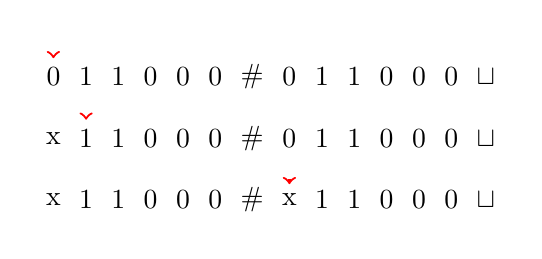
\begin{tikzpicture}[ampersand replacement=\&]
\matrix 
{
  \node(0){};  \&\&\&\&\&\& \& \&\&\&\&\&\& \\
  \node(01){0}; \& \node{1}; \& \node{1}; \& \node{0}; \& \node{0}; \&\node{0}; \&
  \node{\#}; \& 
  \node{0}; \& \node{1}; \& \node{1}; \& \node{0}; \& \node{0}; \& \node{0}; \& \node{$\sqcup$}; \\
    \& \node(1){};  \&\&\&\&\& \& \&\&\&\&\&\& \\
  \node{x}; \& \node(11){1}; \& \node{1}; \& \node{0}; \& \node{0}; \&\node{0}; \&
  \node{\#}; \& 
  \node{0}; \& \node{1}; \& \node{1}; \& \node{0}; \& \node{0}; \& \node{0}; \& \node{$\sqcup$}; \\
\&\&\&\&\&\& \&    \node(2){};   \&\&\&\&\&\& \\
  \node{x}; \& \node{1}; \& \node{1}; \& \node{0}; \& \node{0}; \&\node{0}; \&
  \node{\#}; \& 
  \node(21){x}; \& \node{1}; \& \node{1}; \& \node{0}; \& \node{0}; \& \node{0}; \& \node{$\sqcup$}; \\
};
\draw [->,red,thick] (0) -- (01) ;
\draw [->,red,thick] (1) -- (11) ;
 \draw [->,red,thick] (2) -- (21) ;
% \draw [->,red,thick] (1.center) -- (a) ;
\end{tikzpicture}
\item
  formal-level: all detailed transitions
\end{enumerate}
\item We will mainly use high-level descriptions later

\end{itemize}\end{frame} \begin{frame}[allowframebreaks] \frametitle{Example 3.23}

  \begin{equation*}
  A=
\{\langle  G\rangle \mid G:\mbox{connected undirected graph}\}
\end{equation*}
  \begin{itemize}
\item A high-level TM
  \begin{enumerate}
  \item Mark a node in G
  \item Repeat until no new nodes marked
  \item [] \label{item:1}\qquad For every node $G$, mark it if $\exists$ an edge
to a 
\item [] \qquad marked node
\item If all nodes marked: accept, otherwise: reject
  \end{enumerate}

\item Real implementation

\item [] Figure 3.24

  \begin{center}
    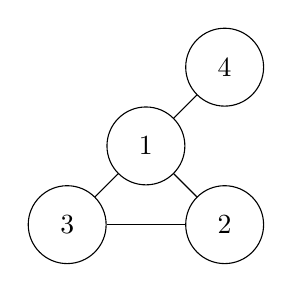
\begin{tikzpicture}
[inner sep=2.5mm]      
\path ( 0,0) node (3) [shape=circle,draw] {3}
( 2,0) node (2) [shape=circle,draw] {2}
( 2,2) node (4) [shape=circle,draw] {4}
( 1,1) node (1) [shape=circle,draw] {1};
\draw [-] (1) -- (2);
\draw [-] (2) -- (3);
\draw [-] (1) -- (3);
\draw [-] (1) -- (4);
\end{tikzpicture}
\end{center}


$\langle  G\rangle=(1,2,3,4)((1,2),(2,3),(3,1),(1,4))$

The input string
\item Details

check nodes distinct: example 3.12:

$E=\{\#x_1\# x_2 \cdots \# x_l\mid x_i \in 
\{0,1\}^*, x_i \neq x_j\}$

end of nodes ? ``)'' used

edges from nodes: similar

stage 1: first node with ``dot''

stage 2: 
\begin{enumerate}
\item find undotted $n_1$ (underline)
\item find dotted $n_2$ (underline)
\item edge $\Rightarrow $ dot $n_1$
\item no edge $\Rightarrow$ next dotted $n_2$

$\vdots$

next undotted $n_1$
\end{enumerate}

stage 4:  scan, check if all nodes dotted

Yes, accept, no: reject

\end{itemize}\end{frame} 

\end{document}

%%% Local Variables:
%%% mode: latex
%%% TeX-master: t
%%% End:
